
\begin{multicols}{2}
A l'aide de la figure ci-contre, on
  cherche à déterminer la longueur $MN$. Les données connues sont
  indiquées sur la figure : $AM=m$; $AN=n$ et
  $\widehat{MAN}=\alpha$. Dans le triangle $ANM$, $H$ est le pied de
  la hauteur issue de $M$.
  \begin{enumerate}
    \item Exprime les longueurs $MH$ et $AH$ en fonction de $m$ et $\alpha$.
    \item Exprime la longueur $NH$ en fonction de $m$, $n$ et
      $\alpha$.
    \item Déduis l'expression de $MN^2$ en fonction de $m$, $n$ et $\alpha$.
  \end{enumerate}
 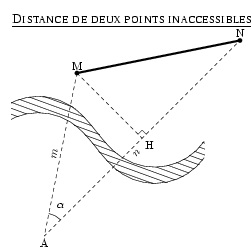
\includegraphics[scale=1]{TR-216.png}  
  \end{multicols}